\section{Implementation}
\label{Section:Implementation}

Section~\ref{Section:RelatedWork} set out what the reviewed literature leaves open. This section describes what was built in response: the environment the agent trades in, the agent itself, and the procedure by which it was trained and a single model chosen for each currency pair.

The order is deliberate. An agent cannot be described apart from the environment that supplies its observations and charges it for its actions, and no number produced by it means anything unless that environment is faithful. The framework therefore comes first, the agent second, and the experimental procedure third.

\subsection{Trading Framework: The Environment the Agent Trades In}
\label{Subsection:TradingFramework}

No framework was available that could both train an agent offline on quote-level history and run that same agent on a live account without rewriting it. Building one took a substantial part of the effort behind this work, and the design choices in it determine what the results in Section~\ref{Section:ExperimentalResults} are worth. Three properties were required. The tested system and the deployed system had to be the same code, so that a result obtained offline says something about live behaviour. The data had to be fine enough to reconstruct the price path inside a bar, because that path decides what a position actually paid. And the costs had to be the costs of a real account rather than a modelling convenience.

\subsubsection{System Architecture: Three Execution Contexts}

The framework is split across two languages by necessity. Strategy logic, the learning models and the market abstractions are written in Python, where the numerical and machine learning libraries are. Access to the broker is written in C\#, because cTrader \cite{noauthor_forex_nodate} executes algorithmic strategies as cBots on the .NET runtime and offers no other route to its order book. The two halves communicate through named memory-mapped files with paired auto-reset event handles, one pair for each direction, operating as a single-slot request and response exchange: the platform writes an update and signals, Python reads it, writes an action and signals back, and the platform proceeds. Two message families cross that boundary, updates travelling from the platform to Python and actions travelling the other way. Figure~\ref{Figure:SystemArchitecture} shows the arrangement. What matters is not the transport but the consequence of it: the strategy object is unaware of where its updates originate. The same class, holding the same weights, runs in three contexts.

\begin{figure}[htb!]
\centering
\begin{tikzpicture}[
  node distance=6mm,
  box/.style={draw, rounded corners=2pt, align=center, font=\small, minimum height=8mm, inner sep=3pt},
  wide/.style={box, text width=34mm},
  narrow/.style={box, text width=26mm},
  lbl/.style={font=\scriptsize\itshape},
  flow/.style={-stealth, thick},
  dashflow/.style={-stealth, thick, dashed}
]
\node[wide] (broker) {Broker\\\scriptsize IC Markets, raw spread, swap-free};
\node[wide, below=of broker] (platform) {cTrader platform};
\node[wide, below=of platform] (cbot) {Connector cBot\\\scriptsize C\# / .NET};
\node[narrow, right=14mm of cbot] (bridge) {Shared memory\\\scriptsize updates $\rightarrow$\\\scriptsize $\leftarrow$ actions};
\node[wide, right=14mm of bridge] (library) {Python library};
\node[narrow, above=8mm of library] (market) {Market abstractions\\\scriptsize ticks, bars, indicators};
\node[narrow, above=8mm of market] (strategy) {Strategy\\\scriptsize DDPG agent};
\node[narrow, below=8mm of library] (portfolio) {Portfolio\\\scriptsize orders, positions, costs};
\node[wide, below=14mm of cbot] (database) {Market database\\\scriptsize PostgreSQL, quote level};

\draw[flow] (broker) -- (platform);
\draw[flow] (platform) -- (cbot);
\draw[flow] (cbot) -- (bridge);
\draw[flow] (bridge) -- (library);
\draw[flow] (library) -- (market);
\draw[flow] (market) -- (strategy);
\draw[flow] (library) -- (portfolio);
\draw[flow] (platform.east) to[out=0, in=90] (bridge.north);
\draw[dashflow] (database) -| (library);
\node[lbl, below=1mm of database] {offline replay bypasses the platform};
\end{tikzpicture}
\caption{Framework architecture. The strategy receives updates and returns actions without knowing whether they originate from a live account, from the platform's own backtester, or from the stored quote database.}
\label{Figure:SystemArchitecture}
\end{figure}

In the first context the platform is absent. Python replays stored quotes directly from the market database, which is the fastest of the three and the one used for training and for every result reported in this work. In the second the strategy runs inside cTrader's own backtesting tab against the platform's historical data, which serves as an independent check on the offline engine. In the third the same strategy runs on a live account, receiving real quotes and sending real orders. The value of this arrangement is that the three contexts differ only in the source of the updates. A strategy that behaves one way in a backtest and another when deployed is usually the product of two separate implementations that drifted apart; here there is one implementation, and the question does not arise.

\subsubsection{Market Data: Collection, Storage and Resolution}

The historical data was collected through the same connector, requested from cTrader by the C\# component and written to a local PostgreSQL database by the Python one. Two record types are stored. Ticks hold the bid and ask quoted at an instant, together with the conversion rates needed to express a profit or loss in the account currency at that instant. Bars hold open, high, low and close as references to the ticks that produced them, so a bar is a view over the tick tape rather than a separate copy of the prices. Table~\ref{Tables:DataInventory} gives the inventory for the seven pairs. The tick tape is the primary record and the bar series are derived from it, which is what allows the engine to reconstruct the path a price took inside a bar rather than interpolating between its endpoints.

\begin{table}[htb!]
\centering
\footnotesize
\begin{tabular}{@{}lrrrrr@{}}
\toprule
\textbf{Pair} & \textbf{Ticks} & \textbf{M1 bars} & \textbf{H1 bars} & \textbf{D1 bars} & \textbf{MN1 bars} \\
\midrule
AUD/USD & 227,914,614 & 4,643,990 & 78,320 & 3,346 & 150 \\
EUR/USD & 242,847,954 & 4,636,138 & 78,145 & 3,339 & 150 \\
GBP/USD & 281,490,557 & 4,648,216 & 78,311 & 3,339 & 150 \\
NZD/USD & 203,788,307 & 4,631,614 & 78,282 & 3,339 & 150 \\
USD/CAD & 228,356,007 & 4,635,179 & 78,319 & 3,347 & 150 \\
USD/CHF & 194,186,979 & 4,621,503 & 78,307 & 3,338 & 150 \\
USD/JPY & 284,430,458 & 4,638,775 & 78,151 & 3,338 & 150 \\
\midrule
\textbf{Total} & \textbf{1,663,014,876} & \textbf{32,455,415} & \textbf{547,835} & \textbf{23,386} & \textbf{1,050} \\
\bottomrule
\end{tabular}
\caption{Market data collected from cTrader and stored locally, spanning January 2014 to August 2026. The tick tape occupies 295 GB and is the primary record; the bar series reference the ticks that produced them.}
\label{Tables:DataInventory}
\end{table}

Two properties of this data need stating, because both would otherwise look like defects.

Bars are stamped at the close of the broker's trading session rather than at midnight, at 22:00 UTC or 21:00 under daylight saving. A daily series therefore carries five bars in a normal week, stamped Sunday through Thursday, and the bar stamped Thursday is Friday's session. An audit against a calendar-day reference reports every Friday as missing, which is a convention rather than a loss. The period from 11 to 25 January 2016 is absent from all seven pairs, in ticks and in bars alike. The gap is broker-side and was confirmed unrepairable by a re-download that visited those days and returned nothing. It is uniform across the seven pairs, so it does not bias any comparison between them, and it falls outside the evaluation window used in Section~\ref{Section:ExperimentalResults}.

\subsubsection{Cost Model: Spread, Commission and Account Type}

The execution engine advances on ticks rather than on bar closes. A position opened during a bar is filled at a quote that existed within that bar, and a stop or target attached to it is tested against the quotes in the order they arrived. This matters for the reason given in Section~\ref{Section:RelatedWork}: a bar reports four prices and conceals the sequence in which the price visited them, and that sequence decides whether a stop was reached before a target and which spread was crossed.

The account modelled is a swap-free raw-spread retail account, and each of the three charges described in Section~\ref{Subsection:PerformanceMeasurement} is applied at the rate such an account pays. A buy is filled at the ask and a sell at the bid, both read from the tick tape at the instant of the fill, so the spread is charged by construction rather than deducted afterwards. The commission is charged on traded volume at $3.5$ points per side, which for a standard lot of $100{,}000$ units is $3.5$ units of the quote currency per side, or $7$ per round turn. The swap is zero, which on a swap-free account is not an approximation but the rate the account actually charges. Table~\ref{Tables:CostModel} lists the full configuration.

\begin{table}[htb!]
\centering
\footnotesize
\begin{tabularx}{\textwidth}{@{}llX@{}}
\toprule
\textbf{Setting} & \textbf{Value} & \textbf{Meaning} \\
\midrule
Account type & Raw spread, swap-free & An account a retail client can open, quoting the interbank spread and charging no overnight financing \\
\addlinespace
Spread & Accurate & The bid-ask difference recorded at the moment of the trade, read from the tick tape rather than assumed \\
\addlinespace
Commission & 3.5 points per side & Charged on traded volume; equivalently 3.5 units of the quote currency per standard lot per side, or 7 per round turn \\
\addlinespace
Swap & 0 points & The rate a swap-free account charges; not an approximation \\
\addlinespace
Account currency & EUR & Profit and loss converted at the rate recorded on the tick that produced it \\
\addlinespace
Initial balance & 10,000 & Reported across five starting balances, as described in Section~\ref{Section:ExperimentalResults} \\
\addlinespace
Leverage & 30 & The retail limit applicable to major currency pairs \\
\addlinespace
Position mode & Netting & One net position per instrument, rather than independent hedged positions \\
\bottomrule
\end{tabularx}
\caption{Cost and account configuration applied to every evaluation reported in this work.}
\label{Tables:CostModel}
\end{table}

The decision to read the spread rather than assume it is worth defending with the data, because the assumption is common and the error it introduces is not small. Figure~\ref{Figure:SpreadOverTime} plots the monthly mean spread of each pair across the evaluation window. For EUR/USD, the most liquid pair in the market, the monthly mean ranges from $0.77$ to $13.00$ points, a factor of seventeen between the quietest month and the busiest. USD/CHF reaches $37.82$ points in January 2015, when the Swiss National Bank abandoned its floor against the Euro. Across the seven pairs the ratio between the widest and narrowest month is never below five.

\begin{figure}[htb!]
\centering
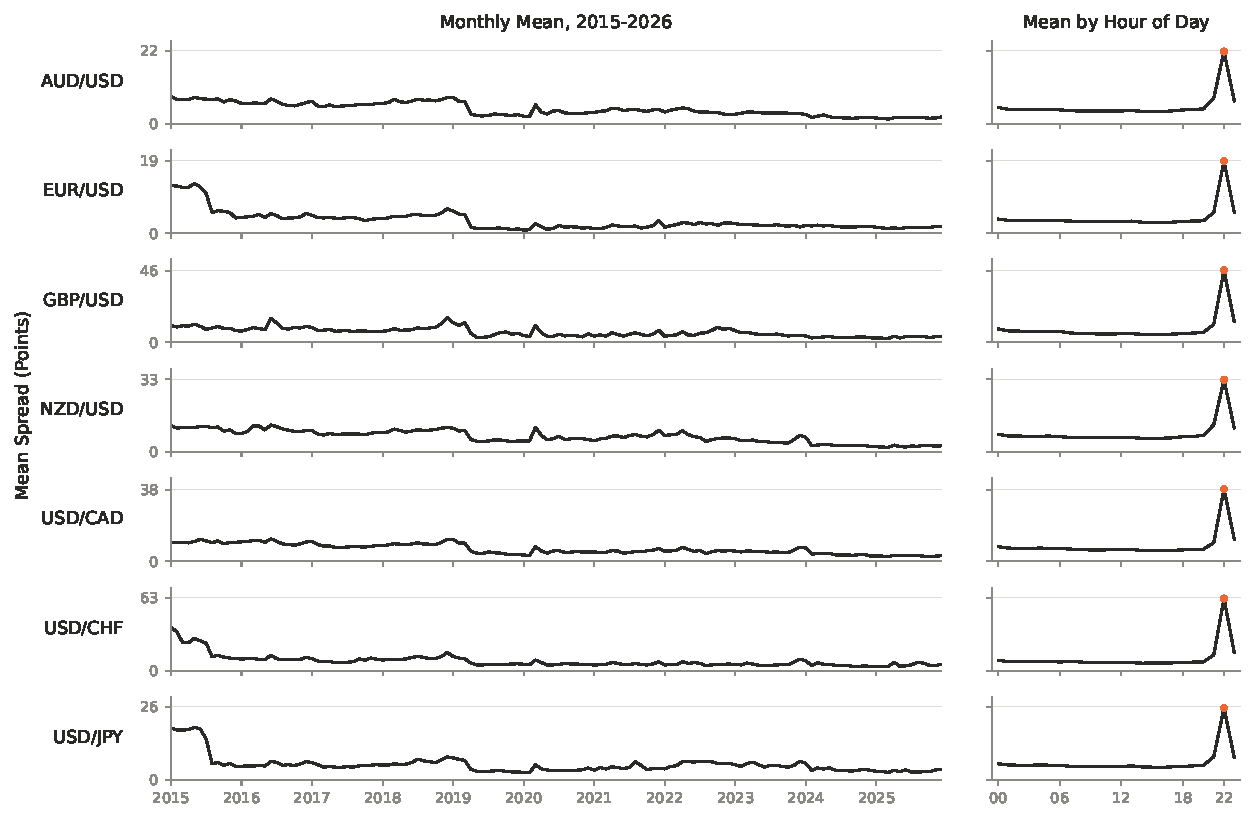
\includegraphics[width=\textwidth]{Images/SpreadOverTime.pdf}
\caption{Monthly mean spread in points for the seven major pairs, 2015 to 2026, computed from the full tick tape. EUR/USD is drawn in black. A model evaluated at a fixed spread is evaluated against a market that exists in no month of this sample.}
\label{Figure:SpreadOverTime}
\end{figure}

The shape of that variation matters more than its size. Spreads widen when liquidity falls and around the events that move prices, which are the moments at which a model trained on an average spread would most expect to act. A strategy charged a constant spread is therefore not merely charged the wrong amount; it is charged the wrong amount in a way that is correlated with its own activity, and the error runs in the direction that flatters it.

The engine was validated against cTrader's own backtester rather than against itself. Across six reference configurations, covering two currency pairs and three windows, its trade, position, order and deal records reproduce the platform's output byte for byte, and the conversion of profit and loss into the account currency was checked independently against the platform's own figures; the only divergence is sub-pip and follows from the resolution of the stored quotes rather than from the accounting. The engine therefore reproduces the platform it was built against, and then goes beyond it. The same strategy is evaluated offline directly on the tick tape, at a speed the platform's own backtester cannot reach and over windows it will not span, under a cost model that can be set to any account the broker offers rather than to the one the terminal happens to be connected to.

Two consequences follow, and both are stated here so that Section~\ref{Section:ExperimentalResults} can be read correctly. The returns reported in this work are net of the spread actually quoted and of a real commission schedule, so they are lower than the same policy would show on bar closes with a fixed or absent spread, and they are not directly comparable with results obtained that way. And because the account is swap-free, no financing term is estimated or omitted; a strategy that holds positions across many nights is charged for exactly what such an account would charge it.

\subsection{Agent Design: Observation, Action and Reward}
\label{Subsection:AgentDesign}

The environment of Section~\ref{Subsection:TradingFramework} supplies prices and charges for trades. Turning it into a reinforcement learning problem requires three further decisions: what the agent sees, what it is allowed to do, and what it is paid for. This subsection states those three and then the algorithm that learns from them. Each decision is reported with the reasoning behind it, because in every case the alternative was tried and behaved worse, and those failures are part of the result.

\subsubsection{Observation Space: Indicators, Encoding and Normalisation}

The agent observes a vector of $38$ values at each hourly bar. Nothing in it is a raw price. A price level carries no information the agent can generalise from, because a policy learned at $1.05$ has no reason to transfer to $1.20$, and eleven years of history spans ranges that differ by more than that. Every feature is therefore a ratio, and the whole observation is dimensionless. Sixteen technical indicators, listed in Table~\ref{Tables:Observation}, supply the market context. They divide into a fast bank describing the last hours to days and a slow bank describing regimes measured in months, so that the agent can distinguish a move within a trend from a change of trend.

\begin{table}[htb!]
\centering
\footnotesize
\begin{tabularx}{\textwidth}{@{}llrX@{}}
\toprule
\textbf{Indicator} & \textbf{Family} & \textbf{Period} & \textbf{Role in the observation} \\
\midrule
ATR & Volatility & 14 & Volatility unit; divides every trend feature and sets the stop distance \\
\addlinespace
RV (fast) & Volatility & 16 & Short-horizon realised volatility; divides the momentum features \\
RV (slow) & Volatility & 480 & Long-horizon realised volatility; its ratio to the fast reading gives the volatility regime \\
\addlinespace
ER & Trend & 120 & Efficiency ratio; how directional recent movement has been, bounded in $[0, 1]$ \\
\addlinespace
ROC Fast & Momentum & 24 & One day \\
ROC Medium & Momentum & 120 & One week \\
ROC Slow & Momentum & 480 & One month \\
ROC Regime & Momentum & 1{,}440 & One quarter \\
ROC Epoch & Momentum & 2{,}880 & Two quarters \\
\addlinespace
SMA Fast & Trend & 24 & One day \\
SMA Medium & Trend & 120 & One week \\
SMA Slow & Trend & 480 & One month \\
SMA Regime & Trend & 1{,}440 & One quarter \\
SMA Epoch & Trend & 2{,}880 & Two quarters \\
SMA Cycle & Trend & 4{,}320 & Three quarters \\
SMA Era & Trend & 5{,}040 & Roughly one year \\
\bottomrule
\end{tabularx}
\caption{The sixteen technical indicators forming the market context of the observation. Periods are in hourly bars. Each moving average contributes two features, its distance from price and its own differential, both in units of the average true range; each momentum reading contributes one, scaled by the movement expected over its lookback.}
\label{Tables:Observation}
\end{table}

The indicator values are encoded as follows, writing $C$ for the bar close, $\sigma_f$ and $\sigma_s$ for the fast and slow realised volatilities, $A$ for the average true range, and $M_i$ for the $i$-th moving average with period $N_i$:

\begin{equation}
\frac{A}{C}, \qquad \sigma_f, \qquad \ln\!\left(\frac{\sigma_f}{\sigma_s}\right), \qquad \text{ER}
\label{Equation:VolatilityFeatures}
\end{equation}

\begin{equation}
\frac{\text{ROC}(N_j)}{\sigma_f \sqrt{N_j}}, \qquad \frac{C - M_i}{A}, \qquad \frac{M_i - M_i^{-1}}{A}
\label{Equation:TrendFeatures}
\end{equation}

Each construction removes a different dependence. Dividing the average true range by the close expresses volatility as a fraction of price. The logarithm of the fast to slow volatility ratio is a volatility regime indicator that is zero when the two agree, positive when volatility is rising and negative when it is falling. Dividing a momentum reading by $\sigma_f \sqrt{N_j}$ scales it by the movement that would be expected over that lookback under a random walk, so that a value near one means a move of ordinary size regardless of the period. Measuring the distance from a moving average in units of the average true range states how far price sits from its trend in terms of the volatility currently being experienced, and the differential of the same quantity gives the direction that trend is moving. The remaining features are the calendar position encoded as four sine and cosine pairs, the current signed exposure as a fraction of the maximum the account could hold, and six values describing the last bar as log returns of its open, high, low and close against the previous close, divided by $\sigma_f$.

Features that are not bounded by construction are standardised by a causal exponentially weighted z-score with $\alpha = 1/200$. Writing $x_t$ for a raw value and $\mu_t$, $s^2_t$ for its running mean and variance:

\begin{equation}
z_t = \frac{x_t - \mu_{t-1}}{\sqrt{s^2_{t-1} + \epsilon}}
\label{Equation:Normalisation}
\end{equation}

\begin{equation}
\mu_t = \mu_{t-1} + \alpha \delta_t, \qquad s^2_t = (1 - \alpha)\left(s^2_{t-1} + \alpha \delta_t^2\right), \qquad \delta_t = x_t - \mu_{t-1}
\label{Equation:NormalisationUpdate}
\end{equation}

The subscript $t-1$ in Equation~\ref{Equation:Normalisation} is the point of the design. A value is standardised using statistics that end at the previous step, and only afterwards is it folded into those statistics. A z-score computed over the whole sample would leak the future into every observation and inflate every result derived from it. Features already bounded, such as the exposure fraction, the efficiency ratio and the calendar encodings, carry a flag that bypasses this layer so that their natural range is preserved.

\subsubsection{Action Space: Position Sizing and Risk}

The agent emits a single continuous value $a \in [-1, 1]$. Its sign is the direction of the position and its magnitude is the fraction of a reference size to hold, so direction and size are one decision rather than two. This is the property that the discrete action sets surveyed in Section~\ref{Section:RelatedWork} cannot express. The reference size is fixed-fractional. Writing $B$ for the account balance, $\rho$ for the risk fraction per position and $k$ for the stop distance in multiples of the average true range, the reference volume $V_{ref}$ is the volume that loses $\rho B$ if price moves $k \cdot A$ against it, and the target volume is that reference scaled by the action:

\begin{equation}
V_{target} = a \cdot V_{ref}, \qquad V_{ref} = \frac{\rho \, B}{k \, A}
\label{Equation:PositionSizing}
\end{equation}

with $\rho = 1\%$ and $k = 1.5$ throughout. The agent therefore never chooses an absolute number of units; it chooses a fraction of a size that the risk rule has already set, and that size shrinks automatically as volatility rises.

One defect in this arithmetic was found during the campaign and is reported here because it affects one of the seven results. The conversion between the quote currency and the account currency is absent from the volume calculation, so the risk actually taken is $\rho / p$ rather than $\rho$, where $p$ is the price of the pair. For pairs quoted near unity the difference is immaterial, and the six pairs quoted against the US Dollar all take approximately the intended $1\%$. For USD/JPY, quoted near $120$ at the start of the sample, the effective risk is $0.008\%$, small enough that the computed volume falls below the broker's minimum and no position can open at all. The compensation applied was to scale $\rho$ by the price, restoring the intended risk per position rather than adding leverage; Section~\ref{Section:ExperimentalResults} reports the level used for each pair. The underlying defect is a limitation of the framework rather than of the method, and it is recorded as future work.

\subsubsection{Reward Function: Log Return, Scaling and Clipping}

The reward at each step is the log return of account equity, scaled and then clipped:

\begin{equation}
r_t = \operatorname{clip}\!\left(\lambda \ln\!\frac{E_t}{E_{t-1}},\; -c,\; +c\right), \qquad \lambda = 1000, \quad c = 1
\label{Equation:Reward}
\end{equation}

The log return is the natural choice for a trading objective because it is additive over time: the per-step rewards telescope to $\ln(E_T / E_0)$, so maximising their sum maximises terminal compounded wealth, and it is independent of account size. The scale factor is not cosmetic, and the reason is a result rather than a convenience. Risk-adjusted rewards of the differential kind described by Moody and Saffell, in which an online estimate of a Sharpe or Sortino ratio is accumulated, are scale-invariant: doubling every position leaves the ratio unchanged. An agent optimising such a reward receives no gradient pushing its position size upward, and in this environment it collapses to roughly $3\%$ of the size available to it, producing a policy that is directionally sensible and financially pointless. A scale-sensitive reward is therefore necessary, and $\lambda$ raises an hourly equity log return, typically of order $10^{-4}$, to a magnitude the critic can resolve against its own approximation error.

The clip is a numerical safeguard of the kind introduced with the Deep Q-Network \cite{mnih_human-level_2015}, applied after the encoding. Its effect here should be stated plainly rather than left implicit, because $\lambda$ and $c$ are not independent: together they clip the raw log return at $\pm c / \lambda = \pm 0.1\%$. On the delivered EUR/USD model the bound is reached on $38.2\%$ of the $68\,155$ hourly steps, with a median absolute scaled reward of $0.70$. For roughly two steps in five the agent is therefore told the direction of the equity move but not its magnitude. That is a real property of the objective, and it is reported here so that the learned behaviour in Section~\ref{Section:ExperimentalResults} is read against the reward the agent actually received.

\subsubsection{Learning Algorithm: DDPG and its Adaptations}

The algorithm is the Deep Deterministic Policy Gradient of Section~\ref{Subsection:DeepReinforcementLearning}, with the actor, critic and their delayed targets as described there, trained from a replay buffer with Ornstein-Uhlenbeck exploration noise. The equations of that section are not repeated. What follows are the six respects in which the implementation departs from the original, each with the reason, and Table~\ref{Tables:Hyperparameters} sets every value against the published one.

\begin{table}[htb!]
\centering
\footnotesize
\begin{tabularx}{\textwidth}{@{}llll X@{}}
\toprule
\textbf{Parameter} & \textbf{Original} & \textbf{This work} & \textbf{Status} & \textbf{Reason for the difference} \\
\midrule
Actor hidden layers & $400 \times 300$ & $64 \times 32$ & Changed & Noisy, non-stationary series supports less capacity \\
Discount factor $\gamma$ & $0.99$ & $0.9995$ & Changed & Horizon matched to the holding period, months rather than days \\
Hidden normalisation & Batch & Layer & Changed & Single-observation inference must match batched training \\
\addlinespace
Actor learning rate & $10^{-4}$ & $10^{-4}$ & Unchanged & \\
Critic learning rate & $10^{-3}$ & $10^{-3}$ & Unchanged & \\
Soft update rate $\tau$ & $0.001$ & $0.001$ & Unchanged & \\
Batch size $N$ & $64$ & $64$ & Unchanged & \\
Replay capacity & $10^{6}$ & $10^{6}$ & Unchanged & \\
Critic weight decay & $10^{-2}$ & $10^{-2}$ & Unchanged & \\
Noise $\theta$, $\sigma$ & $0.15$, $0.2$ & $0.15$, $0.2$ & Unchanged & \\
Final layer init & $U[-3\!\times\!10^{-3}, 3\!\times\!10^{-3}]$ & same & Unchanged & \\
\addlinespace
Gradient clip & --- & $1.0$ & Added & Bounds a single update against a rare large error \\
Warmup transitions & --- & $3{,}000$ & Added & First updates drawn from a varied buffer \\
Actor penalty $\beta$ & --- & $0.001$ & Added & Prevents saturation of the output tangent and constant-action collapse \\
Reward scale $\lambda$ & --- & $1{,}000$ & Added & Lifts an hourly log return above the critic's approximation error \\
Reward clip $c$ & --- & $1$ & Added & Numerical safeguard; bounds the raw log return at $\pm 0.1\%$ \\
\bottomrule
\end{tabularx}
\caption{Hyperparameters against the original Deep Deterministic Policy Gradient \cite{lillicrap_continuous_2015}. Three values were changed, five mechanisms were added, and the remainder are the published ones.}
\label{Tables:Hyperparameters}
\end{table}

The first departure is the observation and the reward, described above.

The second is the size of the networks. The original uses hidden layers of $400$ and $300$ units for low-dimensional control tasks; here they are $64$ and $32$. A $38$-dimensional observation over a noisy, non-stationary series supports far less capacity than a physics simulator with a clean reward, and larger networks fitted the training window without transferring. The third is the discount factor, raised from $0.99$ to $0.9995$. At an hourly step $\gamma = 0.99$ gives a horizon of about a hundred bars, roughly four days, which is shorter than the positions this strategy is intended to hold. At $0.9995$ the horizon extends to some two thousand bars, on the order of three months, which matches the regime indicators in the observation.

The fourth is normalisation inside the networks. The original applies batch normalisation to the hidden layers; this implementation applies layer normalisation instead. The reason is deployment. Batch normalisation behaves differently on a single sample than on a training batch, because it depends on running statistics accumulated during training, and the agent must act on exactly one observation at a time when it runs on a live account. Layer normalisation normalises across the features of one sample, so the computation performed during training is the computation performed in deployment, and the target networks do not carry a second set of running statistics that must be kept synchronised.

The fifth is gradient clipping. The original specifies none; here the gradient norm of both the actor and the critic is clipped to $1$ before each optimiser step. This bounds the size of a single update and prevents a rare large temporal-difference error from moving the parameters far enough to destabilise the critic. It is a stability measure and nothing more; in particular it does not address the collapse discussed next, which is caused by an absence of gradient rather than an excess of it.

The sixth is a penalty on the actor. This is the one change that alters the objective rather than its optimisation, and it exists because the algorithm as published does not train on this problem. The actor's final layer applies a hyperbolic tangent to a pre-activation $u(s)$ to bound the action, and the derivative of that function vanishes as $|u|$ grows. If the policy is driven into that region it stops responding: the action saturates at $\pm 1$, no gradient flows back, and the agent holds one constant position for the remainder of training. The remedy is to penalise the magnitude of the pre-activation directly, which keeps the policy inside the responsive region of the tangent:

\begin{equation}
L_{actor} = -\frac{1}{N}\sum_{i} Q\!\left(s_i, \tanh u(s_i) \,\middle|\, \theta^{Q}\right) + \frac{\beta}{N}\sum_{i} u(s_i)^2
\label{Equation:ActorRegularisation}
\end{equation}

\begin{figure}[htb!]
\centering
\resizebox{\textwidth}{!}{%
\begin{tikzpicture}[
  node distance=5mm,
  layer/.style={draw, rounded corners=1.5pt, align=center, font=\scriptsize, minimum height=9mm, inner sep=3pt, text width=20mm},
  point/.style={draw, circle, inner sep=1.5pt, font=\scriptsize},
  flow/.style={-stealth, semithick},
  pen/.style={-stealth, semithick, dashed}
]
\node[layer] (s) {observation\\$s \in \mathbb{R}^{38}$};
\node[layer, right=of s] (h1) {Linear 64\\LayerNorm\\ReLU};
\node[layer, right=of h1] (h2) {Linear 32\\LayerNorm\\ReLU};
\node[layer, right=of h2] (f3) {Linear 1};
\node[point, right=6mm of f3] (u) {$u$};
\node[layer, right=6mm of u] (th) {$\tanh$};
\node[layer, right=of th] (a) {action\\$a \in [-1,1]$};
\node[font=\scriptsize, below=8mm of u, align=center] (pen) {penalty $\beta\,\overline{u^{2}}$};

\draw[flow] (s) -- (h1);
\draw[flow] (h1) -- (h2);
\draw[flow] (h2) -- (f3);
\draw[flow] (f3) -- (u);
\draw[flow] (u) -- (th);
\draw[flow] (th) -- (a);
\draw[pen] (pen) -- (u);
\end{tikzpicture}}
\caption{The actor. Layer normalisation replaces the batch normalisation of the original, so a single observation is processed exactly as a training batch is. The penalty of Equation~\ref{Equation:ActorRegularisation} acts on the pre-activation $u$, before the tangent, which is where saturation would otherwise remove the gradient.}
\label{Figure:ActorNetwork}
\end{figure}

with $\beta = 0.001$. Setting $\beta = 0$ recovers the original actor loss exactly, so the change is a strict extension rather than a substitution. Together with the scale-sensitive reward, this is what prevents policy collapse; the two mechanisms address different halves of the same failure, the reward supplying a gradient that rewards larger positions and the penalty keeping the actor in the region where that gradient can act. Everything else follows the published algorithm. The learning rates, the soft update rate, the batch size, the replay capacity, the exploration noise parameters, the critic weight decay and the layer initialisation are the values given in the original work, and a warmup period of $3000$ transitions is used before learning begins so that the first updates are drawn from a buffer with some variety in it rather than from the first few correlated steps of an episode.

\subsection{Experimental Procedure: Training, Selection and Deployment}
\label{Subsection:ExperimentalProcedure}

An agent design does not by itself produce a result. Training is stochastic, so the same configuration run twice gives two different policies, and a procedure is needed that says which of them is reported and on what grounds. This subsection describes that procedure, the criteria applied at each stage, and the two deployment decisions that sit between the learned policy and the orders actually sent.

\subsubsection{Training Procedure: Seeds, Episodes and Data Splits}

The eleven-year window is divided once into three consecutive periods. Writing the window as $[T_0, T_3)$ with $T_0$ the first of January 2015 and $T_3$ the first of January 2026:

\begin{equation}
\underbrace{[T_0, T_1)}_{\text{training, 9 years}} \quad
\underbrace{[T_1, T_2)}_{\text{validation, 1 year}} \quad
\underbrace{[T_2, T_3)}_{\text{testing, 1 year}}
\label{Equation:Split}
\end{equation}

Weights are updated on the training period only. The validation period decides which state of the network is kept. The testing period is visited once, after every other decision has been taken. Within that split, a single training run proceeds as follows. A seed fixes the network initialisation, the exploration noise stream and the order in which the replay buffer is sampled, and thereby determines the entire run. The agent then performs $30$ episodes, an episode being one pass over the training period. Weights are not reset between episodes: the run is a single trajectory of $30$ passes, and the network at the start of episode $n+1$ is the network at the end of episode $n$. After each episode the agent is evaluated once over the validation period with learning disabled, and that evaluation is reduced to a single number by the Calmar ratio, its annualised return divided by its maximum drawdown. Writing $f_n$ for that value and $g_n$ for an eligibility test defined below, the state retained after episode $n$ is

\begin{equation}
\theta^{\star} \leftarrow \theta_n \quad \text{if} \quad (g_n \wedge \neg g^{\star}) \;\vee\; \left(g_n = g^{\star} \wedge f_n > f^{\star}\right)
\label{Equation:KeepBest}
\end{equation}

which keeps an eligible episode over an ineligible one regardless of score, and otherwise keeps the higher score within the same eligibility class. The saved state is a copy: the run continues training from $\theta_n$, not from $\theta^{\star}$, so a later episode is never restarted from an earlier checkpoint. The eligibility test $g_n$ rejects policies that are degenerate rather than merely poor. An episode qualifies only if it opened at least ten positions, spent at least three hundred bars on each side of the market, and held its weaker side for at least $30\%$ of the time it held its stronger one. A policy that never trades, or that is long for the entire period, can produce a respectable Calmar ratio on a trending window while having learned nothing about when to hold a position, and the test removes it from consideration before the score is compared. Between $128$ and $256$ seeds were run for each currency pair, differing in nothing but the seed. Figure~\ref{Figure:TrainingPipeline} shows how the three stages fit together.

\begin{figure}[htb!]
\centering
\begin{tikzpicture}[
  node distance=5mm,
  stage/.style={draw, rounded corners=2pt, align=center, font=\small, text width=32mm, minimum height=8mm, inner sep=3pt},
  small/.style={stage, font=\scriptsize, text width=30mm},
  note/.style={font=\scriptsize\itshape, align=left},
  flow/.style={-stealth, thick}
]
\node[stage] (seed) {Seed $s$\\\scriptsize init, noise, sampling};
\node[small, right=10mm of seed] (episode) {Episode $n$ of 30\\one pass over training};
\node[small, right=10mm of episode] (valid) {Validation pass\\learning disabled};
\node[small, below=9mm of valid] (keep) {Calmar $f_n$ + eligibility\\keep-best checkpoint};
\node[small, below=9mm of episode] (test) {Test pass\\once, after 30 episodes};
\node[stage, below=9mm of seed] (pool) {Pool of 128--256\\trained seeds};
\node[stage, below=9mm of pool] (gates) {Gates\\reject degenerate};
\node[small, right=10mm of gates] (sweep) {Risk sweep\\$\times 1.0$ to $\times 3.0$};
\node[small, right=10mm of sweep] (score) {Composite score\\percentile ranks};
\node[stage, below=9mm of gates] (champion) {Published model};

\draw[flow] (seed) -- (episode);
\draw[flow] (episode) -- (valid);
\draw[flow] (valid) -- (keep);
\draw[flow] (keep) -- node[note, above, midway] {} (test);
\draw[flow] (keep.west) to[out=180, in=0] node[note, above, midway] {\scriptsize next episode} (episode.south east);
\draw[flow] (test) -- (pool);
\draw[flow] (pool) -- (gates);
\draw[flow] (gates) -- (sweep);
\draw[flow] (sweep) -- (score);
\draw[flow] (score.south) to[out=270, in=0] (champion.east);
\end{tikzpicture}
\caption{The three stages of the procedure. The Calmar ratio chooses among episodes within one seed; the composite score of Section~\ref{Subsection:ExperimentalProcedure} chooses among seeds.}
\label{Figure:TrainingPipeline}
\end{figure}

One property of this arrangement must be stated explicitly, because it limits what the results in Section~\ref{Section:ExperimentalResults} can claim. The split of Equation~\ref{Equation:Split} governs the training of an individual seed. The choice of which seed to publish, described next, is made on performance measured over the whole eleven-year window, and the performance figures reported in this work are measured over that same window. The testing period is therefore held out from the training of each candidate and from the choice among its episodes, but not from the choice among candidates, and the headline returns are not out-of-sample estimates. This is the weakest point in the method and it is not disguised anywhere in what follows.

\subsubsection{Model Selection: Gates and Composite Ranking}

Once the seeds for a pair have been trained, each is evaluated over the full window under the cost model of Table~\ref{Tables:CostModel}, and one is chosen. The choice is made in two steps, rejection followed by ranking, because the two questions are different: whether a policy is admissible at all, and which of the admissible ones is best.

Four gates reject a candidate outright. Its return must be positive. Its weaker direction must account for at least $10\%$ of its exposure, which removes policies that are long or short throughout. Its mean holding period must be at least twenty-four bars, which removes policies whose signal is noise. And its regime score, the fraction of market movement during which it was positioned correctly, must exceed the score its own policy achieves when its position sequence is rotated in time. That last gate deserves a note, because a fixed threshold was tried first and does not work. A rotated policy holds the same positions for the same durations but at the wrong moments, so its score measures what that policy's autocorrelation and holding structure would earn by luck alone. Measured across the seven pairs those nulls range from $48$ to $70$, so a fixed bar of, say, $55$ would be below chance on one pair and needlessly severe on another. The null is therefore computed per model rather than assumed.

Candidates surviving the gates are ranked by a composite of percentile ranks within their own pool. For a metric $m$ and a pool of $K$ candidates, the rank of candidate $i$ is

\begin{equation}
R_m(i) = 100 \cdot \frac{\left|\left\{ j : v_m(j) < v_m(i) \right\}\right|}{K - 1}
\label{Equation:PercentileRank}
\end{equation}

where $v_m$ is negated for metrics that are better when smaller, such as drawdown. The metrics are divided into three groups, listed in Table~\ref{Tables:Composite}, and the score is the unweighted mean of the three group means:

\begin{equation}
S(i) = \frac{1}{3} \sum_{G \in \{\text{money}, \text{safety}, \text{behaviour}\}} \frac{1}{|G|} \sum_{m \in G} R_m(i)
\label{Equation:Composite}
\end{equation}

\begin{table}[htb!]
\centering
\footnotesize
\begin{tabularx}{\textwidth}{@{}lX@{}}
\toprule
\textbf{Group} & \textbf{Metrics, each entering as a percentile rank within the candidate pool} \\
\midrule
Money & Annualised return, Calmar ratio, Sterling ratio \\
\addlinespace
Safety & Sharpe ratio, Sortino ratio, inverse maximum drawdown, inverse downside volatility \\
\addlinespace
Behaviour & Two-sidedness (the weaker exposure side as a fraction of half), regime edge over the model's own rotation null, mean holding period, longest holding period \\
\bottomrule
\end{tabularx}
\caption{Components of the composite selection score of Equation~\ref{Equation:Composite}. The three groups carry equal weight, so return contributes one ninth of the total rather than dominating it. The ratios are those defined in Section~\ref{Subsection:PerformanceMeasurement}.}
\label{Tables:Composite}
\end{table}

Two design decisions are embedded in Equation~\ref{Equation:Composite}. Ranks are relative to the pool rather than absolute, so no threshold can exclude a candidate that is simply better than everything around it. And the three groups carry equal weight, so a policy cannot win on return alone: money, safety and behaviour each contribute a third, and a candidate with the highest return in its pool but no two-sidedness and no regime edge scores poorly on two groups out of three. Each surviving candidate is also evaluated at several position sizes, from the reference risk of Equation~\ref{Equation:PositionSizing} up to three times it. Scaling the risk fraction does not change the learned policy, only the size of the positions it takes, and the level chosen for each pair is reported with the results.

\subsubsection{Deployment: Decision Cadence and Rebalance Threshold}

Two decisions separate the learned policy from the orders that are actually sent, and between them they account for more of the delivered performance than any hyperparameter.

The first is the decision cadence. The agent observes every hourly bar, but it is permitted to act only once per calendar day. A key is formed from the timestamp of each bar and a new action is committed only when that key changes:

\begin{equation}
\kappa(t) = (\text{year}(t), \text{month}(t), \text{day}(t))
\label{Equation:DecisionKey}
\end{equation}

The key is built from the calendar rather than from a count of bars, which makes it robust to the gaps and short sessions described in Section~\ref{Subsection:TradingFramework}: a week containing a holiday still produces one decision per trading day rather than drifting out of alignment. The second is a rebalance threshold. A continuous action changes slightly at every decision, and acting on every such change would send a stream of tiny orders each paying the spread and a commission. An order is therefore sent only when the change in the target position is large enough to be worth its cost:

\begin{equation}
\left| V_{target} - V_{current} \right| \;\geq\; \max\!\left(V_{min},\; \eta \left| V_{ref} \right|\right), \qquad \eta = 0.20
\label{Equation:Hysteresis}
\end{equation}

where $V_{min}$ is the broker's minimum volume. The threshold is a fraction of the reference volume rather than of the position currently held, so it does not vanish as a position is reduced. Table~\ref{Tables:Deployment} isolates the contribution of each decision, measured on one model with nothing retrained. The comparison is between four configurations of the same weights, so the differences are attributable to the deployment layer alone.

\begin{table}[htb!]
\centering
\footnotesize
\begin{tabular}{@{}llrrrr@{}}
\toprule
\textbf{Cadence} & \textbf{Threshold} & \textbf{Commission} & \textbf{Return} & \textbf{Sharpe} & \textbf{Max drawdown} \\
\midrule
Daily & --- & none & $+42.48\%$ & $0.319$ & $24.4\%$ \\
Hourly & --- & none & $-38.57\%$ & $-0.308$ & $50.5\%$ \\
Hourly & --- & 3.5 points & $-64.70\%$ & $-0.732$ & $70.5\%$ \\
Daily & $0.20$ & 3.5 points & $+34.02\%$ & $0.275$ & $23.5\%$ \\
\bottomrule
\end{tabular}
\caption{Contribution of the two deployment decisions, measured on one EUR/USD model over the full window with nothing retrained. All four rows are the same weights under different execution settings, so the differences are attributable to the deployment layer alone. This model precedes the seven-pair campaign and serves here only to isolate the effect.}
\label{Tables:Deployment}
\end{table}

Two things follow from that table. Moving from hourly to daily decisions is worth some eighty percentage points, turning a losing configuration into a profitable one, because an hourly cadence acts on noise the eleven-year horizon of the discount factor was never meant to capture. And the rebalance threshold recovers roughly twelve percentage points under realistic costs while reducing drawdown rather than increasing it, which is unusual: commission alone costs over twenty percentage points without the filter and about six with it. A continuous action space is what makes the strategy expressive, and this filter is what makes it affordable.

\subsubsection{Worked Example: One Position From Decision to Settlement}

The preceding subsections define each component separately. This one follows a single position through all of them, using a trade taken by the delivered EUR/USD model, so that the arithmetic can be checked rather than assumed.

At 02:00 on 30 January 2019 the daily decision key of Equation~\ref{Equation:DecisionKey} changed, and the agent was consulted for the first time that day. It received the 38-value observation of Section~\ref{Subsection:AgentDesign}, built from the bar that had just closed, and returned a positive action. The reference volume of Equation~\ref{Equation:PositionSizing} at that moment, risking $1\%$ of the balance over a stop of $1.5$ average true ranges, gave a target of $12{,}000$ units of the base currency once the action had scaled it and the result was rounded to the broker's volume step. The change from the position then held exceeded the threshold of Equation~\ref{Equation:Hysteresis}, so an order was sent. The tick recorded at that instant quoted $1.14392$ ask against $1.14387$ bid, a spread of five points. The buy was filled at the ask. Twenty-four hours later the key changed again, the agent's action reversed the sign, and the position was closed at the bid then quoted, $1.14931$. The profit follows from those two prices and the volume, and is expressed in the account currency at the conversion rate recorded on the closing tick:

\begin{equation}
12{,}000 \times \left(1.14931 - 1.14392\right) = 64.68 \text{ USD} \;\;\longrightarrow\;\; 56.27 \text{ EUR}
\label{Equation:WorkedGross}
\end{equation}

The spread is already inside that figure. It was paid at entry by filling at the ask rather than the mid, and again at exit by filling at the bid, which is what makes the round trip cross it exactly once. The commission is charged separately at both ends:

\begin{equation}
2 \times 3.5 \times 10^{-5} \times 12{,}000 = 0.84 \text{ USD} \;\;\longrightarrow\;\; 0.72 \text{ EUR}
\label{Equation:WorkedCommission}
\end{equation}

The swap is zero, the position having been held overnight on a swap-free account. The position therefore settled at $56.27 - 0.72 = 55.55$ EUR, which is the figure recorded in the exported trade record. One trade says little. Across all $1{,}777$ trades the delivered EUR/USD model took over the eleven years, the same accounting gives a gross profit of $8{,}733.62$ EUR, a commission charge of $1{,}669.50$ EUR and a swap charge of exactly zero, for a net of $7{,}064.12$ EUR. Commission alone consumed $19.1\%$ of the gross profit, and that is before the spread, which is not separable from the gross figure because it is embedded in every fill. A result reported without these charges would be describing a different strategy.

Everything described here was fixed before any result was seen: one architecture, one observation, one reward, one selection rule, applied unchanged to seven instruments. That constraint is what makes the outcomes comparable across pairs.

It also makes them falsifiable. A design tuned until it works on a single instrument can always be made to work on that instrument, and nothing in its results distinguishes a strategy from a description of that instrument's history. Applying the same design to seven leaves it nowhere to hide, and the results in Section~\ref{Section:ExperimentalResults} include a pair on which it does not work.